\documentclass[conference]{IEEEtran}
\usepackage[T1]{fontenc}
\usepackage{mathptmx}
\usepackage{amsmath,amssymb,graphicx,booktabs,url}
\usepackage[hidelinks]{hyperref}
\title{Card Fraud Triage via Gaussian Mixture Density Scoring\\Phase 1: Machine Learning Evaluation}
\author{\IEEEauthorblockN{Team T085}\IEEEauthorblockA{Section E, Project 26\\Rishihood University}}
\begin{document}
\maketitle
\begin{abstract}
We study card fraud as novelty detection using the original ULB/Kaggle dataset. All models learn from 170,528 legitimate training records under frozen chronological partitions. An expanded train-only search compares seven component counts and four covariance types, followed by predetermined optimizer trials. The selected full-covariance GMM has 20 components and achieves test average precision 0.5822. At the 0.5\% validation false-positive-rate budget it catches 57 of 75 test frauds with 175 false positives. We add 26 validation-only sensitivity fits across dimension, covariance, random seed and training size, explicit saved split membership, and post-freeze error analysis. The same test set was inspected in an earlier run, so these expanded results are follow-up findings rather than a fresh independent holdout. Autoencoder and hybrid training remain Phase 2.
\end{abstract}
\begin{IEEEkeywords}
fraud triage, novelty detection, Gaussian mixture, EM, precision-recall, chronological evaluation
\end{IEEEkeywords}

\section{Introduction}
Fraud review is constrained by investigator capacity. A useful model should place fraud near the top of a manageable queue while limiting legitimate transactions flagged for review. Because the original dataset contains only 492 frauds among 284,807 records, majority prediction gives approximately 99.827\% accuracy while detecting none of the fraud. We therefore emphasize ranking quality, false positives and workload rather than accuracy.

Our central question is whether modeling normal transaction density provides useful triage under chronological evaluation. A GMM permits multiple modes of legitimate behavior, but low density does not necessarily imply fraud. We compare it with PCA reconstruction, Isolation Forest and an approximate one-class support-vector method. The same legitimate-only training set supports every model. We keep the required GMM baseline even when a comparator performs better.

This report addresses Phase 1 machine learning evaluation only. The overall project title includes an autoencoder, but no neural model or hybrid claim is included in the completed experiments. The expanded study adds persisted split membership, a broader train-only GMM search, validation-only robustness studies and descriptive error analysis. The original test partition has already been inspected; the expanded results explicitly disclose that reuse.

\section{Related Work}
Dempster, Laird and Rubin describe expectation-maximization for incomplete-data maximum likelihood, including mixture models \cite{em}. In our setting component identity is latent. EM supplies a fitting procedure; convergence alone does not validate an anomaly detector.

Liu, Ting and Zhou introduce Isolation Forest, which scores anomalies through random partition isolation rather than a fitted Gaussian density \cite{iforest}. It provides a comparator with a different structural assumption. Our forest has 200 trees with 256 sampled observations per tree.

Saito and Rehmsmeier motivate precision-recall evaluation for imbalanced classification \cite{pr}. We use AP as the primary ranking summary and report trapezoidal PR area separately. Operational thresholds supplement those summaries by measuring how much fraud a concrete review policy captures.

PCA reconstruction provides a linear subspace comparator. The approximate one-class SVM uses a Nystr\"om RBF feature map and SGDOneClassSVM. These are fixed classical baselines, not test-tuned optimizers. Full-covariance GMMs, in contrast, estimate density along several local covariance directions. This comparison tests whether density fit translates into useful fraud ranking.

\section{Dataset and Quality Checks}
The original ULB/Kaggle credit card fraud CSV \cite{data} contains 284,807 observations, 31 columns and 492 fraud labels. It supplies V1--V28, provider-created anonymized PCA features, alongside Time, Amount and Class. The observed Time range is 0--172,792 seconds. Our input audit finds no missing or non-finite cells, no negative Time or Amount values, and 1,081 exact duplicate records.

We retain exact duplicates because transaction identifiers are absent and repeated records cannot be reliably classified as ingestion errors. Since Time is part of an exact duplicate and tied times remain together, exact duplicate rows cannot cross our split boundaries. Retention can still overweight repeated behavior within partitions. A deduplication sensitivity experiment is future work.

\begin{table}[t]
\caption{Chronological partitions of the original CSV.}
\centering\small
\begin{tabular}{lrrr}\toprule
Split & Rows & Fraud & Fraud rate \\\midrule
Train & 170,888 & 360 & 0.21066\% \\
Validation & 56,958 & 57 & 0.10007\% \\
Test & 56,961 & 75 & 0.13167\% \\\bottomrule
\end{tabular}\label{tab:split}
\end{table}

The file is stably sorted by Time and split near 60/20/20 by record count. Boundaries move to the right edge of equal timestamps. Training ends at 120,396 seconds, validation spans 120,397--145,248 seconds, and test spans 145,249--172,792 seconds. These are unequal-duration windows. The different class prevalences in Table~\ref{tab:split} show that random-split intuition should not be assumed.

Exploratory plots use only the training partition. We inspect class balance, log-amount distributions, time distributions and feature correlations. Training descriptive statistics are exported for inspection. The current test metric computation follows the model and threshold freeze. However, this test partition was already inspected in the initial Phase 1 run; it is reused here and is not a new independent holdout.

\begin{figure}[t]
\centering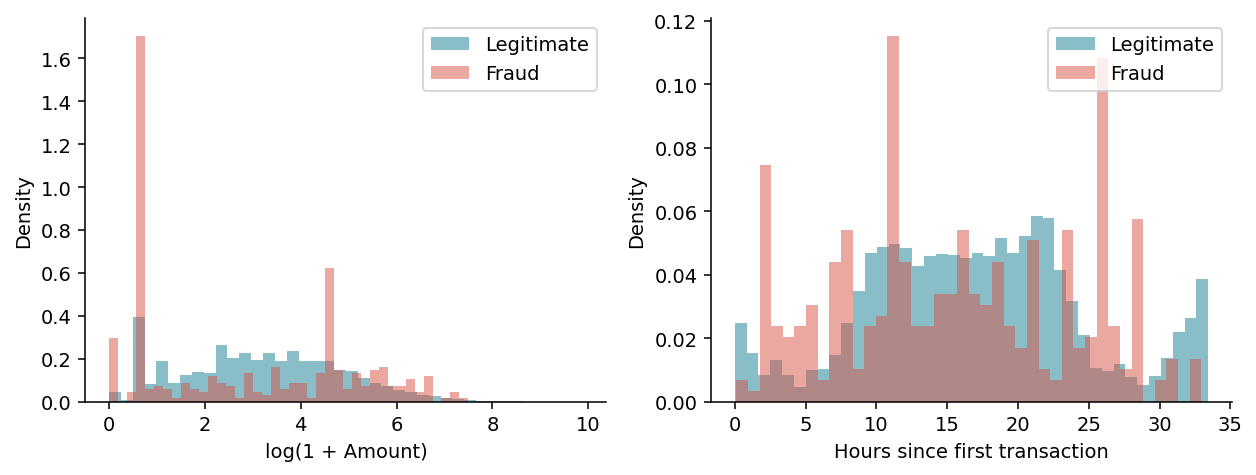
\includegraphics[width=\columnwidth]{figures/eda_amount_time.png}
\caption{Training-only log-amount and time distributions. Density normalization makes the rare fraud distribution visible without implying equal class frequency.}
\end{figure}

\section{Feature Engineering and Leakage Control}
Inputs comprise V1--V28 and $\log(1+\mathrm{Amount})$, for $d=29$. The monotone log transform compresses the nonnegative amount scale. StandardScaler learns means and standard deviations from legitimate training observations only. For feature $j$,
\begin{equation}
z_{ij}=\frac{g_j(x_{ij})-\mu_{j,\mathrm{train},0}}{\sigma_{j,\mathrm{train},0}},
\end{equation}
where $g_j$ is identity except for Amount. The same transformation is applied to validation and test.

Time is used for ordering and EDA but excluded from model features. A monotonically increasing elapsed-time coordinate could label later observations anomalous simply because they occur later. Only two days are available to support alternative periodic encodings. Class is never part of the input matrix. Training labels identify known legitimate records, so this is clean-normal novelty detection rather than a procedure with no label access whatsoever.

No oversampling, SMOTE or random train/test shuffling is used. The upstream anonymizing PCA was already applied by the dataset provider. Its fitting provenance cannot be independently audited or reproduced with the released features; our leakage controls apply to transformations learned within this project.

\section{Gaussian Mixture Theory and Application}
\subsection{Density and score}
A $K$-component density is
\begin{equation}
p(\mathbf z)=\sum_{k=1}^{K}\pi_k\mathcal N(\mathbf z\mid\boldsymbol\mu_k,\boldsymbol\Sigma_k),
\quad \pi_k\geq0,\ \sum_k\pi_k=1.
\end{equation}
We use $s(\mathbf z)=-\log p(\mathbf z)$ so all model scores increase with anomalousness. Continuous density is not a fraud probability and may exceed one. Posterior component membership likewise is not posterior fraud risk.

\subsection{Expectation-maximization}
At the E-step, component responsibilities are
\begin{equation}
r_{ik}=\frac{\pi_k\mathcal N(\mathbf z_i\mid\boldsymbol\mu_k,\boldsymbol\Sigma_k)}{\sum_l\pi_l\mathcal N(\mathbf z_i\mid\boldsymbol\mu_l,\boldsymbol\Sigma_l)}.
\end{equation}
With $N_k=\sum_i r_{ik}$, the M-step updates
\begin{align}
\pi_k&=N_k/n,\\
\boldsymbol\mu_k&=N_k^{-1}\sum_i r_{ik}\mathbf z_i,\\
\boldsymbol\Sigma_k&=N_k^{-1}\sum_i r_{ik}\boldsymbol\delta_{ik}\boldsymbol\delta_{ik}^T+\lambda\mathbf I,\quad\boldsymbol\delta_{ik}=\mathbf z_i-\boldsymbol\mu_k.
\end{align}
The structural grid initially sets $\lambda=10^{-5}$, allows 300 iterations and uses two initializations; staged trials then vary these settings. EM can converge to different local solutions. Regularization helps prevent singular covariance, but it does not remove all sensitivity to initialization or narrow density directions.

\subsection{Model selection and staged optimization}
The structural search crosses $K\in\{1,2,4,8,12,16,20\}$ with diagonal, full, tied and spherical covariance. All 28 candidates fit identical legitimate training observations in the same 29-dimensional feature space. For $p$ free parameters and training likelihood $L$,
\begin{equation}
\mathrm{AIC}=2p-2\log L,\qquad\mathrm{BIC}=p\log n-2\log L.
\end{equation}
Full covariance has $(K-1)+Kd+Kd(d+1)/2$ parameters, diagonal $(K-1)+2Kd$, tied $(K-1)+Kd+d(d+1)/2$, and spherical $(K-1)+Kd+K$. Minimum finite BIC among converged fits selects the structural anchor. Predetermined one-factor trials at that anchor vary regularization across $10^{-6},10^{-5},10^{-4}$, initialization count across 1,2,3 and iteration cap across 100,300. Duplicate baseline settings are not refitted. This is a staged search rather than a full Cartesian optimization.

Across 33 primary fits, 0 failed or did not converge. The selected model has 20 full-covariance components, $\lambda=10^{-6}$, 2 initialization(s) and an iteration limit of 300. Its BIC is -13246003.8 and AIC -13339427.6. AIC and BIC select the same recorded fit. A minimum at the largest tested K is a bounded-search result, not a global optimum claim.

The selected model's maximum covariance condition number is 17759113.4 and minimum component weight is 0.0019. EM convergence does not by itself establish stability. Negative information criteria are possible for continuous density. Neither validation fraud labels nor test metrics select the primary GMM. Information criteria are not compared across the dimensionality and sample-size studies because the feature spaces or fitting populations differ.
\begin{figure}[t]
\centering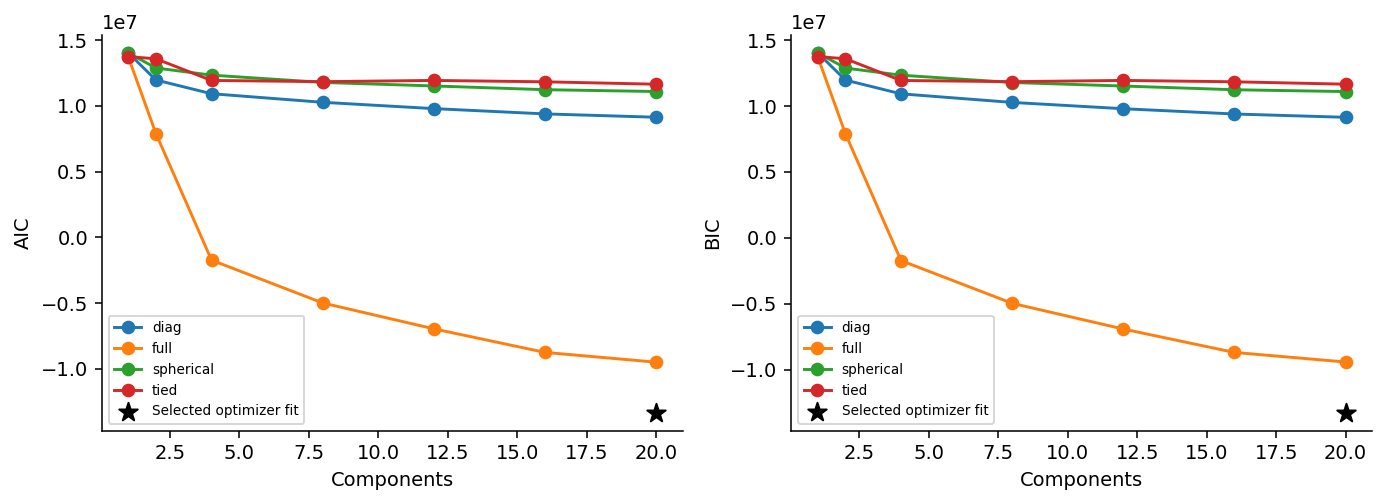
\includegraphics[width=\columnwidth]{figures/gmm_selection.png}
\caption{Training AIC and BIC for structural candidates. The star marks the selected optimizer fit; all trial diagnostics appear in the selection table.}
\end{figure}

\section{Classical Comparators}
Isolation Forest receives the full legitimate training matrix, with its built-in subsampling of 256 records per tree. Its anomaly score is the negative of scikit-learn's normality score. PCA uses 15 components with full SVD and scores mean squared reconstruction error across standardized inputs.

The approximate one-class SVM maps inputs to 128 Nystr\"om RBF features, using $\gamma=1/29$. A second StandardScaler and SGDOneClassSVM with $\nu=0.01$ fit those features using the same normal training records. The random seed is 26, maximum SGD iterations are 2,000, and tolerance is $10^{-4}$. This approximates an RBF one-class boundary while avoiding exact kernel scaling on over 170,000 observations. It must not be described as exact OC-SVM.

Baseline settings are fixed, with no test-driven tuning. We omit LOF and exact kernel OC-SVM to keep full-data fitting practical. Accordingly, this study establishes results for the implemented fixed configurations, not exhaustive superiority over every classical detector.

\section{Evaluation Protocol}
\subsection{Ranking summaries}
Report AP, trapezoidal PR AUC and secondary ROC AUC. AP weights precision by recall increments; trapezoidal PR area linearly connects curve points \cite{ap}. The no-skill precision reference uses each partition's own fraud prevalence. Test prevalence is 0.001317.

The GMM AP interval is 0.4634--0.7123, from 500 stratified bootstrap resamples retaining class counts. These descriptive intervals omit temporal dependence, prevalence changes and model-refitting uncertainty. They are not a paired superiority test.

\subsection{Frozen false-positive policies}
For budget $\alpha$, sort legitimate validation scores descending and let $m=\lfloor\alpha n_0\rfloor$. Use the zero-indexed score at rank $m$ as threshold and flag strictly larger scores. This permits at most $m$ validation false positives, conservatively handling ties. Budgets are 0.1\%,0.5\%,1\%,5\%. Freeze cutoffs before test labels are evaluated, then report realized test FPR rather than assuming exact transfer. Store hexadecimal float cutoffs and reload them exactly, avoiding decimal-parser rounding at tied boundaries.

\subsection{Review capacity}
Separately review the top $k=\max(1,\lfloor qn\rfloor)$ scores for $q\in\{0.001,0.005,0.01\}$, plus top 100. Stable chronological order breaks score ties. Labels measure quality after scores select the queue. The top-0.5\% test capacity is 284 reviews. This batch policy differs from a frozen scalar threshold.


\section{Results and Operational Trade-offs}
Table~\ref{tab:ranking} reports the fixed comparator configurations and the train-BIC-selected GMM. GMM test AP is 0.5822, compared with PCA 0.1573, Isolation Forest 0.0538, and approximate OC-SVM 0.0014. These results describe these configurations and this reused historical split, not exhaustive superiority of a method family.

GMM ROC AUC is 0.9187, while precision-recall summaries remain sensitive to the rare-event review burden. Approximate OC-SVM's weak result is retained; it does not establish that exact kernel OC-SVM cannot work. Bootstrap intervals do not substitute for a paired significance test.

At the 0.5\% validation FPR policy, GMM's threshold is 63.5486. Test outcomes are TP=57, FP=175, FN=18, TN=56711. Recall is 76.00\%, precision 24.57\%, realized FPR 0.308\%, and total alerts 232. The workload is 3.07 false positives and 4.07 reviews per caught fraud. Other configured policies appear in Table~\ref{tab:policy}.

The separate top-0.5\% policy reviews 284 records and catches 57 frauds, with precision 20.07\% and recall 76.00\%. Top 100 captures 56 frauds. Labels measure queue quality after membership is selected from scores. Frozen thresholds and batch capacity policies can produce different workloads.

\begin{table}[t]
\caption{Test ranking metrics. AP is the primary summary.}
\centering\small
\begin{tabular}{lrrr}\toprule
Model & AP & PR AUC & ROC AUC \\\midrule
% BEGIN GENERATED ranking
GMM & 0.5822 & 0.5787 & 0.9187 \\
Isolation Forest & 0.0538 & 0.0524 & 0.9520 \\
PCA reconstruction & 0.1573 & 0.1540 & 0.9642 \\
Approx. OC-SVM & 0.0014 & 0.0014 & 0.5411 \\
% END GENERATED ranking
\bottomrule\end{tabular}\label{tab:ranking}
\end{table}
\begin{table}[t]
\caption{GMM reused-test outcomes at frozen validation FPR budgets. All rates are percentages.}
\centering\footnotesize
\begin{tabular}{rrrrrr}\toprule
Budget & TP & FP & Recall & Actual FPR & Precision \\\midrule
% BEGIN GENERATED operating
0.1 & 55 & 29 & 73.33 & 0.051 & 65.48 \\
0.5 & 57 & 175 & 76.00 & 0.308 & 24.57 \\
1.0 & 58 & 324 & 77.33 & 0.570 & 15.18 \\
5.0 & 60 & 2082 & 80.00 & 3.660 & 2.80 \\
% END GENERATED operating
\bottomrule\end{tabular}\label{tab:policy}
\end{table}
\begin{figure}[t]
\centering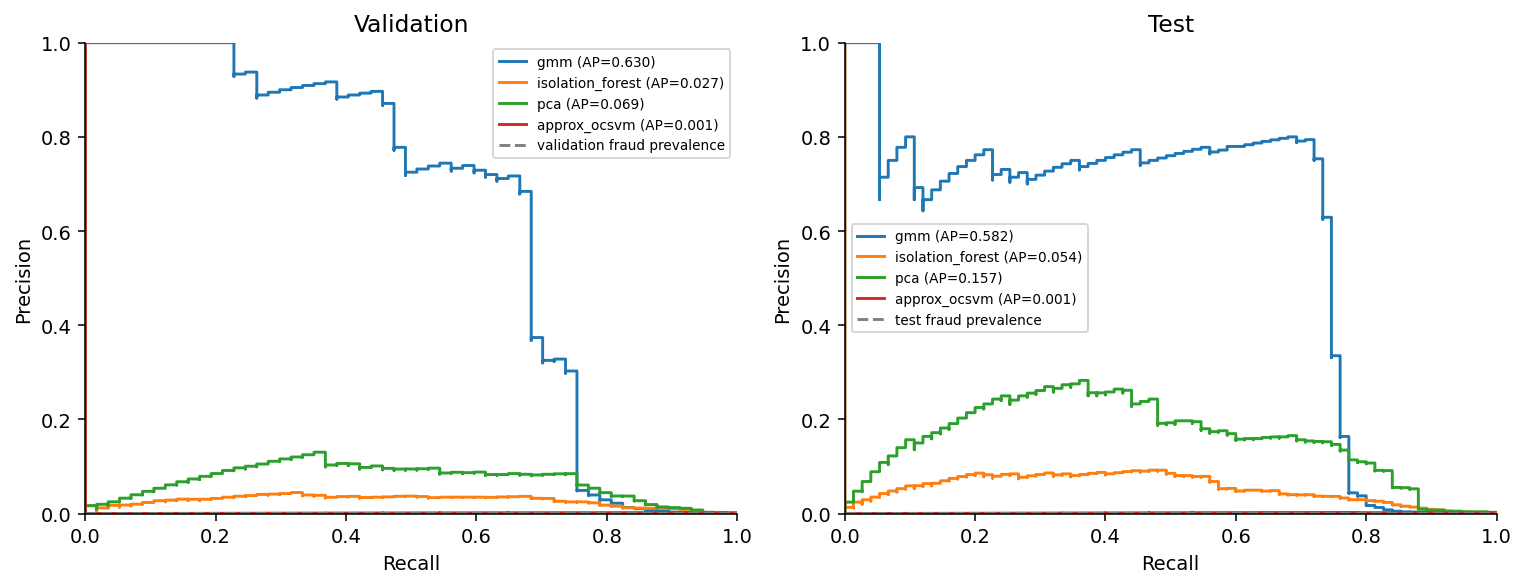
\includegraphics[width=\columnwidth]{figures/pr_curves.png}
\caption{Validation and reused-test PR curves with population-specific prevalence references.}
\end{figure}
\begin{figure}[t]
\centering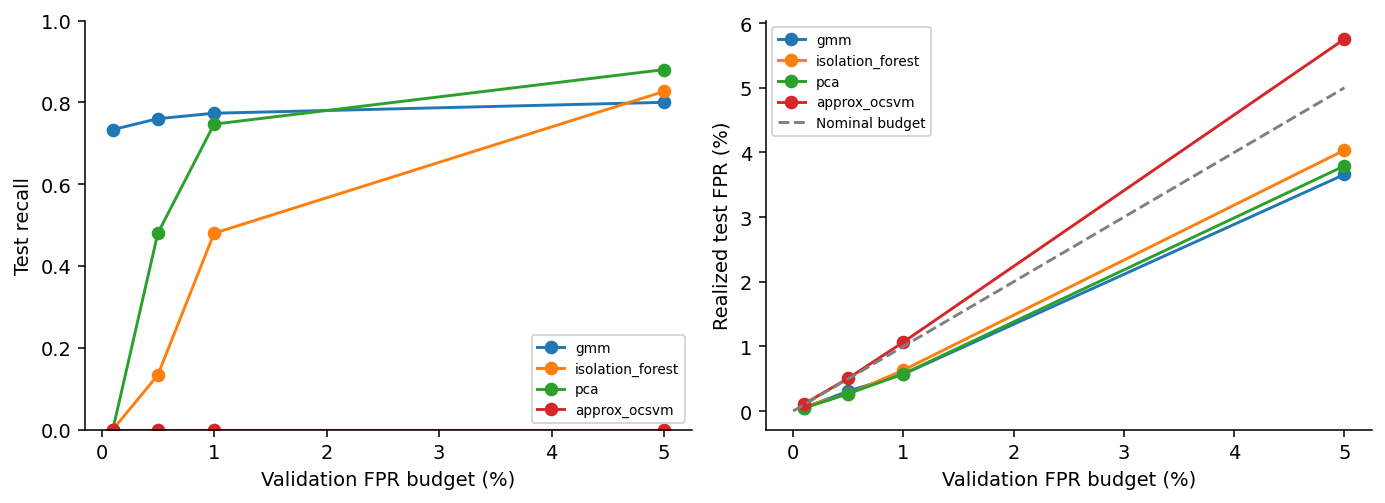
\includegraphics[width=\columnwidth]{figures/threshold_tradeoffs.png}
\caption{Recall and realized test FPR at frozen validation budgets.}
\end{figure}

\section{Reproducibility and Validation}
The source separates data, preprocessing, GMM, baselines, metrics, robustness and error analysis. Seven executed notebooks include an assembled Phase 1 summary. The default \texttt{python run\_all.py} executes the full study. A quick skip-robustness mode is explicitly incomplete for reproduction.

The dataset checksum, chronological indices, legitimate training membership and partition index checksums are persisted. Loading refuses a different dataset, changed fractions, invalid membership or altered chronology. The complete preprocessing pipeline, scaler and study PCA objects are saved locally. Model files are excluded from Git; their regeneration guide remains visible in results/models.

20 automated checks cover chronology, ties, normal-only scaling, pipeline reuse, split provenance/tampering, all covariance forms, logged fit failure, staged selection and metric identities. Package versions, configuration hashes and the test-reuse disclosure are saved. Team responsibilities follow the supplied five-role assignment; actual personal contributions need independent review evidence rather than inferred attribution.


\section{Robustness and Error Analysis}
The validation-only module performs 26 fits. It crosses dimensions 5,10,20,29 with four covariance types at K=4, then repeats full-dimensional covariance settings across seeds 13,26,42 and evaluates nested training subsets. Preprocessing fits only legitimate training rows. No test frame is accepted by this module.

Full-covariance validation AP across dimensions is 5d: 0.0211, 10d: 0.0118, 20d: 0.0085, 29d: 0.0664. 0 diagnostic fits failed or did not converge. All warning and covariance-eigenvalue diagnostics are retained. Condition number above $10^6$ is an explicit diagnostic flag, not a universal validity threshold.

Across the three seeds, covariance-specific AP means and sample standard deviations are diag: 0.0589 $\pm$ 0.0002, full: 0.3534 $\pm$ 0.2488, spherical: 0.0298 $\pm$ 0.0016, tied: 0.1075 $\pm$ 0.0581. Pairwise score-rank correlations range from 0.7170 to 1.0000. Raw-score dispersion is also saved per validation observation. Spherical covariance has condition number one by construction, so conditioning alone cannot establish detector quality.

At training fractions 10\%,50\%,100\%, full-covariance K=4 validation AP is 0.0535, 0.6208, 0.0664. Preprocessing stays fit on the full legitimate training set to isolate GMM sample size. Raw information criteria do not select across these changing populations or dimensions.

Post-freeze test inspection saves every missed fraud, the twenty highest-scoring legitimate alerts, group amount/time/score summaries and standardized feature deviations. These quantities are descriptive, not causal feature explanations. Anonymized features prevent business-semantic interpretation. Error analysis never feeds back into model fitting or threshold choice.
\begin{figure}[t]
\centering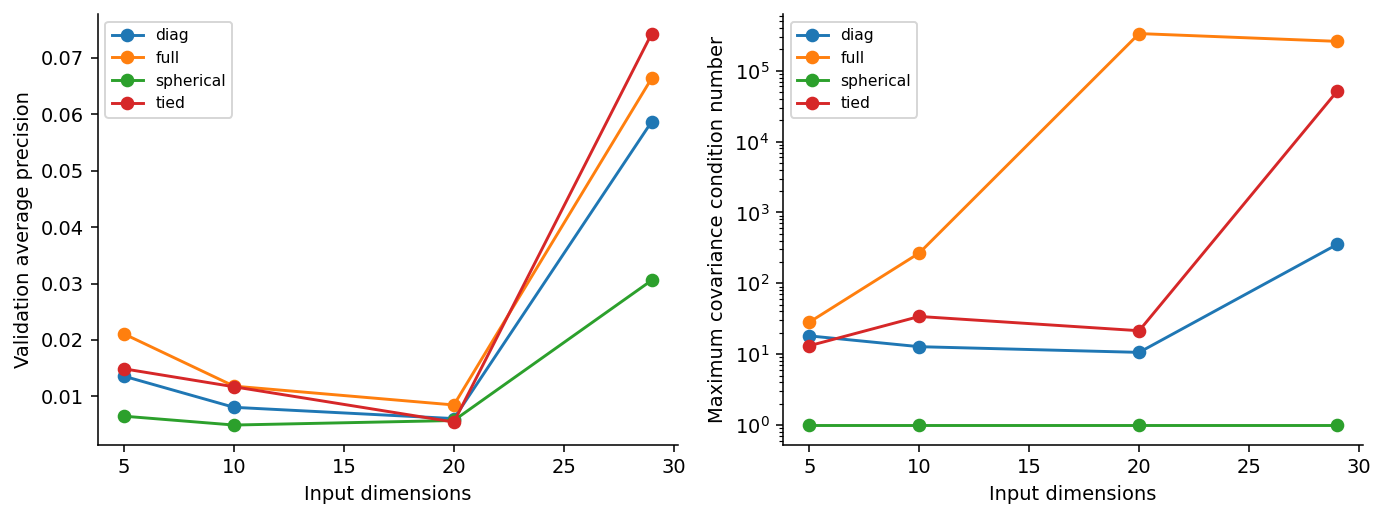
\includegraphics[width=\columnwidth]{figures/dimensionality_stability.png}
\caption{Validation AP and covariance conditioning across dimensionality and covariance assumptions at fixed K=4.}
\end{figure}
\begin{figure}[t]
\centering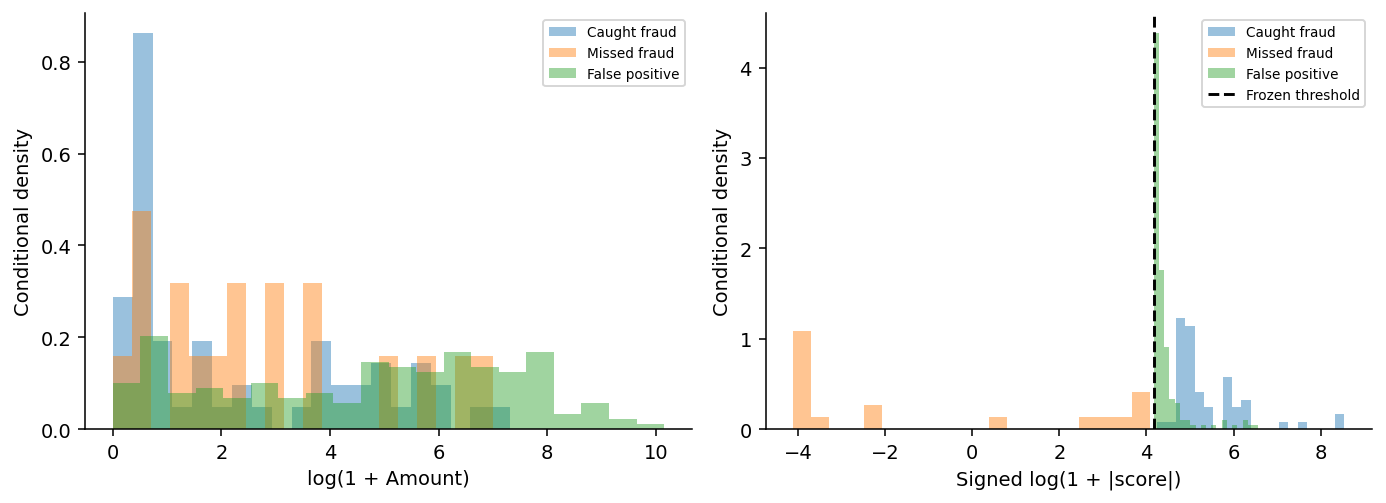
\includegraphics[width=\columnwidth]{figures/error_analysis.png}
\caption{Post-freeze error groups under the 0.5\% validation FPR policy. The score panel uses a monotone signed-log display transform.}
\end{figure}

\section{Limitations and Phase 2 Plan}
Only two historical days and 75 test frauds limit generalization. The test set was already inspected in the initial run; expanded results are follow-up findings. No fresh independent holdout has been obtained. Dataset anonymization, retained duplicates and absent account identifiers limit interpretation and independence analysis.

The search is bounded and staged. The diagnostic studies use fixed K=4, three seeds and a small dimensionality grid; they do not establish universal numerical robustness. Density fit and covariance conditioning do not directly optimize fraud utility. Bootstrap intervals omit temporal dependence, refitting and prevalence uncertainty. Batch review capacity also differs from a streaming queue.

Phase 2 will train an undercomplete or denoising autoencoder using the frozen legitimate training membership and preprocessing. Architecture, early stopping and thresholds must use validation. The model-independent metrics remain the same. Any hybrid needs a rationale and ablation evidence. Continued reuse of this test partition must be disclosed.

\section{Conclusion}
The expanded Phase 1 study combines train-only GMM selection with explicit validation threshold policies, reproducible split membership and documented sensitivity studies. Operational confusion counts and review workload make the trade-offs visible. Validation-only robustness and post-freeze error analysis clarify limitations without treating convergence or low density as proof of fraud. The completed classical pipeline provides the frozen interfaces needed for Phase 2.

\begin{thebibliography}{9}
\bibitem{em} A. P. Dempster, N. M. Laird, and D. B. Rubin, ``Maximum likelihood from incomplete data via the EM algorithm,'' \emph{J. Royal Stat. Soc. B}, vol. 39, no. 1, pp. 1--22, 1977, doi: 10.1111/j.2517-6161.1977.tb01600.x.
\bibitem{iforest} F. T. Liu, K. M. Ting, and Z.-H. Zhou, ``Isolation forest,'' in \emph{IEEE ICDM}, 2008, pp. 413--422, doi: 10.1109/ICDM.2008.17.
\bibitem{pr} T. Saito and M. Rehmsmeier, ``The precision-recall plot is more informative than the ROC plot when evaluating binary classifiers on imbalanced datasets,'' \emph{PLOS ONE}, vol. 10, no. 3, e0118432, 2015, doi: 10.1371/journal.pone.0118432.
\bibitem{data} ULB Machine Learning Group, ``Credit card fraud detection,'' Kaggle. [Online]. Available: \url{https://www.kaggle.com/datasets/mlg-ulb/creditcardfraud}. Accessed Oct. 31, 2026.
\bibitem{ap} Scikit-learn developers, ``average\_precision\_score,'' documentation. [Online]. Available: \url{https://scikit-learn.org/stable/modules/generated/sklearn.metrics.average_precision_score.html}.
\end{thebibliography}
\end{document}
